In this chapter, we explain the relationship between TQC and modular tensor
categories arising from quantum groups. We will focus mainly on the category
$\Fib$ of Fibonacci anyons, which is the simplest MTC which is universal for
quantum computing. 

We will introduce $\Fib$ and discuss in some detail how to simulate the quantum
circuit model in $\Fib$. We will then discuss the universality of this
simulation and algorithms for doing topological quantum computing in practice.

\section{The Fibonacci anyon}
The simplest universal model of TQC, and so a good candidate for implementing
TQC, is the Fibonacci anyon. Here we introduce the Fibonacci anyon and explain
how to simulate quantum circuits using Fibonacci anyons.

The category $\Fib$ of Fibonacci anyons is a modular tensor category which is a
subcategory of $\mathcal{C}^{int}(\sll(2),5)$: its objects are representations
of $U_z^{res}(\sll(2))$ for $z$ a $5^{th}$ root of unity. The simple objects in 
$\Fib$ are $V_0, V_2$. We will refer to them as $\one$ and $\tau$
respectively, $\one$ being the tensor unit and trivial anyon type or vacuum. The
fusion rules in $\Fib$ can be computed easily and are as follows:

\begin{itemize}
    \item $\tau \odot \tau = I \oplus \tau$
    \item $\tau \odot I = \tau$
    \item $I \odot I = I$
\end{itemize}
Recall that the $\oplus$ here means that when $\tau$, $\tau$ fuse, the result
is a superposition of anyons of type $1$ and $\tau$.  The reason they are
called Fibonacci anyons is that $\tau^{\odot n} \simeq F_{n-1} \one \oplus F_{n+2}
\tau$, where $F_n$ is the $n^{th}$ Fibonacci number.

We will now explain a simple way to simulate quantum circuits using Fibonacci
anyons. To simulate quantum circuits, we need

\begin{itemize}
\item Qubits
\item Systems of multiple qubits
\item A way to do measurement
\item Unitary gates
\item A universal gate set
\end{itemize}

First we construct qubits. Consider a triplet $(\tau,\tau,\tau)$ of Fibonacci
anyons. A simple computation shows that 

\begin{equation}
(\tau \odot \tau) \odot \tau \simeq 2\tau \oplus 1
\end{equation}

This means that there are $3$ fusion possibilities for $3$ anyons with type $\tau$:

\newcommand{\fusiondiagram}[2]
{
\begin{pspicture}(0,-0.99125)(2.841875,0.99125)
\psline[linewidth=0.01cm]{->}(0.2209375,0.63)(0.65,0.2)
\psline[linewidth=0.01cm]{->}(1.4209375,0.63)(1.05,0.2)
\psline[linewidth=0.01cm]{->}(0.8209375, -0.12)(1.2209375,-0.57125)
\psline[linewidth=0.01cm]{->}(2.6209376,0.63)(1.5,-0.57125)
\rput(1.531875,0.79875) {$\tau$}
\rput(0.111875,0.79875) {$\tau$}
\rput(2.691875,0.79875) {$\tau$}
\rput(0.85, 0.1)    {$#1$}
\rput(1.35,-0.7)        {$#2$}
\end{pspicture} 
}

\newcommand{\fusiondiagramright}[2]
{
\begin{pspicture}(0,-1)(2.84,1)
\psline[linewidth=0.01cm]{->}(2.62,0.63)(2.19,0.2)
\psline[linewidth=0.01cm]{->}(1.42,0.63)(1.79,0.2)
\psline[linewidth=0.01cm]{->}(2.02,-0.12)(1.62,-0.57)
\psline[linewidth=0.01cm]{->}(0.22,0.63)(1.34,-0.57)
\rput(1.31,0.79875) {$\tau$}
\rput(2.73,0.79875) {$\tau$}
\rput(0.15,0.79875) {$\tau$}
\rput(1.99, 0.1)    {$#1$}
\rput(1.49,-0.7)        {$#2$}
\end{pspicture} 
}

\begin{center}
\label{fusionleft}
\fusiondiagram{\one}{\tau}
\fusiondiagram{\tau}{\one}
\fusiondiagram{\tau}{\tau}
\end{center}

Two of them have the final result $\tau$. We use this fact to define our qubits
to be triples of $\tau$ anyons with total charge $\tau$. We saw in
\ref{fusionleft} that the first two qubits can fuse to be either $\tau$ or
$\one$: denote these two possibilities by $((\tau,\tau)_\one,\tau)_\tau$ and
$((\tau,\tau)_\tau,\tau)_\tau$. 

There is also an equivalent formulation using quadruplets
$((\tau,\tau),(\tau,\tau))_\one$ with total charge $\one$. We use the same
formulation as \cite{Hormozi2007} here.

In $\Fib$, these are represented by eleemnts of $\Hom(\tau, ((\tau \odot
\tau)\odot \tau)) \simeq \Hom(\tau, 2\tau \oplus \one) \simeq \mathbb{C}^2$. 
Define 

\begin{align}
\ket{0} = ((\tau,\tau)_\one , \tau)_\tau \\
\ket{1} = ((\tau,\tau)_\tau , \tau)_\tau 
\end{align}

$\ket{0}$ and $\ket{1}$ are elements of $\Hom(\tau, ((\tau \odot \tau)\odot
\tau))$. We will call $\operatorname{span}\left\{ \ket{0}, \ket{1} \right\}$
the \emph{computational space}. There is also a \emph{noncomputational space}
spanned by $\ket{\text{NC}} = ((\tau,\tau)_\tau,
\tau)_\one$. One of the principal issues with this simulation is that of
``leakage'': some operations take us out of the computational space. 

Performing measurements in the $\left\{ \ket{0}, \ket{1} \right\}$ basis is
straightforward: just fuse the first two anyons and measure the result, then
fuse the remaining two and measure again.

We have explained how 1-qubit systems are simulated. Multiqubit systems are
similar: for $n$ qubits, we take $n$ sets of $3$ anyons: $\tau^{\odot 3n}$.
For $\ket{\varphi},\ket{\psi}\in \Hom(\tau,(\tau \odot \tau) \odot \tau)$,
their tensor product $\ket{\varphi} \odot \ket{\psi} \in \Hom(\tau \odot
\tau, (\tau)^{\odot 6}) \simeq \mathbb{C}^{13}$. 

The vectors $\left\{ \ket{i}\odot \ket{j} : 0 \leq i,j\leq 1 \right\}$
therefore span a 4-dimensional subspace of $\Hom(\tau \odot \tau, (\tau)^{\odot
6}) \simeq \mathbb{C}^{13}$. We again refer to this space as the
\emph{computational space} $V$. As $n$ gets larger, more and more of the space
is the noncomputational space. 

We now turn to the problem of defining gates. $\Fib$ is braided, so for any $n$
and object $V$ in $\Fib$, $B_n$ acts on $\Hom(V, \tau^{\odot n})$ by
composition: 

\begin{equation}
f \mapsto \sigma \circ f
\end{equation}

This gives a representation of the braid group on the hom sets $\Hom(\one,
\tau^{\odot n})$. In fact, it turns out that this representation is unitary.
Braids therefore act unitarily on our qubits, and we will use them as our
quantum gates. How do these braids act? The generator $\sigma_1$ of $B_3$,

\begin{center}
    % drawing of a braid
    \scalebox{1} % Change this value to rescale the drawing.
    {
    \begin{pspicture}(0,-0.9615033)(2.421875,0.9815033)
    \pscustom[linewidth=0.02cm]
    {
    \newpath
    \moveto(0.1609375,0.558031)
    \lineto(0.1309375,0.43743896)
    \curveto(0.1159375,0.37714294)(0.1159375,0.2486859)(0.1309375,0.1805255)
    \curveto(0.1459375,0.112365104)(0.2159375,-0.00822694)(0.2709375,-0.06065797)
    \curveto(0.3259375,-0.113089)(0.4759375,-0.21008728)(0.5709375,-0.25465393)
    \curveto(0.6659375,-0.2992206)(0.8459375,-0.40670472)(0.9309375,-0.4696222)
    \curveto(1.0159374,-0.53253967)(1.1359375,-0.6609961)(1.1709375,-0.726535)
    \curveto(1.2059375,-0.7920746)(1.2459375,-0.87334293)(1.2609375,-0.9205308)
    }
    \pscustom[linewidth=0.02cm]
    {
    \newpath
    \moveto(0.5809375,-0.1340619)
    \lineto(0.7909375,-0.05541505)
    \curveto(0.8959375,-0.01609193)(1.0309376,0.10187865)(1.0609375,0.1805255)
    \curveto(1.0909375,0.25917235)(1.1359375,0.39811522)(1.1809375,0.5790033)
    }
    \pscustom[linewidth=0.02cm]
    {
    \newpath
    \moveto(0.4409375,-0.25989687)
    \lineto(0.2909375,-0.40146118)
    \curveto(0.2159375,-0.47224304)(0.1159375,-0.6216724)(0.0909375,-0.70031923)
    \curveto(0.0659375,-0.77896667)(0.0509375,-0.8785858)(0.0809375,-0.9415033)
    }
    \rput(0.111875,0.7890033){$\tau$}
    \rput(1.151875,0.7890033){$\tau$}
    \rput(2.271875,0.7890033){$\tau$}
    \psline[linewidth=0.02cm](2.2609375,0.59900326)(2.2609375,-0.90099674)
    \end{pspicture} 
    }
\end{center}

acts on $\Hom(\tau, ((\tau \odot \tau) \odot \tau))$ via the unitary matrix

\begin{equation}
\begin{pmatrix}
e^{\frac{-4\pi i}{5}} & 0 \\
0 & e^{\frac{-2\pi i}{5}}  \\
\end{pmatrix}
\end{equation}

with respect to the basis $\left\{ \ket{0}, \ket{1} \right\}$. This can be
computed either using the ``universal $R$-matrix'' in \ref{section:braiding} or
by solving for it using the fusion rules and the axioms for a braided monoidal
category (see \cite{Panangaden}).

$\Hom(\tau, \tau^{\odot 3})$ also has the basis \{ $(\tau,
(\tau,\tau)_\one)_\tau$, $(\tau, (\tau,\tau)_\tau)_\tau$ \}. It is obtained
from the basis $\left\{ \ket{0}, \ket{1} \right\}$ by composing with the
associativity isomorphism $\alpha_{\tau,\tau,\tau}$. The change of basis matrix
is called the \emph{$F$-matrix}. It is

\begin{equation}
\begin{pmatrix}
\phi^{-1} & \sqrt(\phi^{-1}) \\
\sqrt(\phi^{-1}) & -\phi^{-1} \\
\end{pmatrix}
\end{equation}

where $\phi$ is the golden ratio. The $F$-matrix is also unitary.

The $R$ and $F$-matrices allow us to compute the $2 \times 2$ matrix
corresponding to each element of $B_3$ in this representation: the other
generator $\sigma_2$ of $B_3$ acts as $F^{-1}RF$. In fact, the $R$ and $F$
matrices are enough to compute the matrix associated to any element of the
$B_n$ acting on $\Hom(\one, \tau^{\odot n})$ or $\Hom(\tau, \tau^{\odot n})$.


\section{Universality and implementations}

We have explained a standard way to simulate the circuit model using
Fibonacci anyons. It turns out that this is universal:
Freedman et al prove in \cite{Freedman2000} that the image of
$B_6$ in its representation on $Hom(\tau \oplus \tau, \tau^{\odot 6}) \simeq
\mathbb{C}^5 \oplus \mathbb{C}^8$ is dense in $SU(5) \oplus SU(8)$. It follows
that any $2$-qubit unitary gate can be approximated by some braid in $B_6$,
with as little leakage into the noncomputational space as required. 

%There are two issues: firstly it is necessary to find braids $\sigma$ such that
%$\rho(\sigma)$ (at least approximately) takes vectors in the computational
%space to vectors in the computational space. Once this is solved, we need to be
%implement arbitrary unitary gates on the computational space.

This theorem does not however give a means of finding a braid whose image
approximately realizes a given unitary gate. In this section we review how this
problem has been approached.

The most naive solution to the problem of ``topological quantum
compiling'' is brute force search: try braids until one is found where the
image is close enough to the gate required.

In \cite{Hormozi2007}, Hormozi et al reduce the problem of implementing a
universal gate set to that of implementing arbitrary single-qubit gates.
They do this by giving an explicit method for constructing an approximation to
a CNOT gate. They further show how to construct a CNOT gate while only moving
one quasiparticle, which has obvious practical significance.

The first construction of the CNOT gate works as follows. First, find a braid
which approximates the identity, but where the first and third quasiparticles
swap places. The example given is

\begin{center}
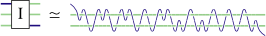
\includegraphics{I-small.png}
\end{center}

and a braid approximating $X$:


\begin{center}
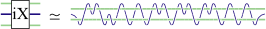
\includegraphics{X-small.png}
\end{center}

Then combine these as follows to obtain an approximation to the CNOT gate:

\begin{center}
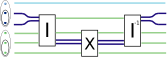
\includegraphics{CNOT-small.png} \\
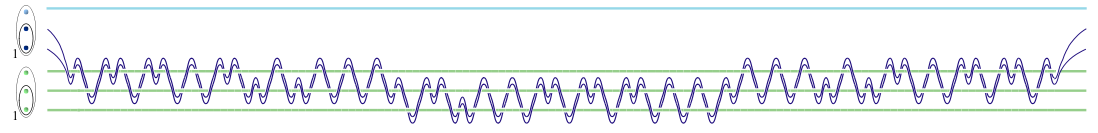
\includegraphics{CNOT-large.png}
\end{center}

When the mobile pair of qubits has total charge $\tau$, the ``identity'' braid
has (approximately) no effect on the system and so the approximate $X$ gate is
applied to the second qubit.

When the mobile pair of qubits has total charge $\one$, the ``identity'' braid
obviously has an effect on the system. Since braiding the tensor unit has no
effect, the overall effect on the system is none at all. So this braid
approximately implements a CNOT gate! In fact, replacing the $X$ gate with any
other gate gives us arbitrary controlled gates.

However, the algorithm for constructing single-qubit gates relies on a
combination of brute force search and the Solovay-Kitaev algorithm.
\cite{Burrello2010},\cite{Burrello2011}, and \cite{Mosseri2008} give an
alternative method using the icosahedral group to approximate single qubit
gates using Fibonacci anyons. 

Burrello et al (\cite{Burrello2010}, \cite{Burrello2011}) use brute-force
search to associate a braid to each icosahedral group element which most
closely approximates it among all braids of length $\leq N$. Call this set
$I(N)$.

They then use $I(N)$ to find a combination of elements of $I(N)$ which is close
to the target gate $T$. This involves another brute force search over the
elements $\left\{ g_1g_2\cdots g_n: g_i \in I(N) \right\}$ for some $n$. 

The approach in \cite{Mosseri2008} is related: no algorithm is given
for approximating particular unitary gates, but rather a method for
approximating increasingly dense meshes in $SU(2)$. The approach here is to
use a brute force search to approximate closely two generators for the
icosahedral group, and then use these two generators to generate a slightly
deformed polytope.

In \cite{Ainsworth2011}, Ainsworth and Slingerland study the general problem of
leakage in topological quantum computing.  In particular, 2 questions are
answered, using only facts about representations of $B_n$:

\begin{enumerate}
\item What is the optimal number of anyons to use to model a qubit?
\item To what extent can leakage be avoided?
\end{enumerate}

To address the first question, they prove that if we use $n > 4$ anyons to
model a qubit, then either:

\begin{itemize}
\item the representation of $B_n$ is abelian
\item there is leakage into the noncomputational space in single qubit operations
\end{itemize}

The mathematical problem that this reduces to is finding the maximum $n$ for
which there is a nonabelian $d$-dimensional representation of $B_n$. A
(nontrivial) theorem shows that the answer is always $d+2$.
Therefore in general for modelling qudits, the same holds if we use $n > d+2$ anyons.

As for the second question, they prove that if there is a system of 2 qubits
where every 2-qubit gate does not cause leakage, then the anyons are Ising
anyons, and therefore not universal.

Further, they show that there are no nonabelian anyons where all the gates on 2
qutrits or 1 qubit + 1 qutrit are leakage-free.

However, if each anyon carries a representation of a quantum group, then their
tensor product does as well and thus all gates are leakage-free. However, it is
conjectured that the braid group representations that occur in this way have
finite image.

Rowell et al conjecture in \cite{Rowell2007} that for any unitary modular
tensor category $\mathcal{C}$, every representation of $B_n$ on the hom sets
has finite image if and only if $\dim_q(X)^2$ is an integer for every simple
object $X$ in $\mathcal{C}$. A verification of this conjecture is given for all
unitary modular tensor categories with $\leq$ 4 simple objects.
       
One interesting question that is so far unanswered is that of whether there are
entangling leakage-free 2-qubit gates in universal quantum models. The work in
\cite{Ainsworth2011} shows us that it is impossible for all gates to be
leakage-free, but the possibility of there being some nontrivial group of such
leakage-free is not excluded. 
